\renewcommand{\vec}[1]{{\boldsymbol #1}}
% \newcommand{\rev}[1]{{\color{red}{#1}}} 
\renewcommand{\comment}[1]{[{\color{blue}{#1}}]} 
% \newcommand{\rev}[1]{{{#1}}} 
\def\nn{\nonumber\\}

% \DeclareMathOperator{\sgn}{sgn}
\newcommand{\cind}[3]{c^{(#1)}_{#2}(#3)}
\newcommand{\cdag}[3]{{c^\dagger}^{(#1)}_{#2}(#3)}
\newcommand{\phind}[3]{\phi^{(#1)}_{#2}(#3)}
\newcommand{\sigmap}{\sigma^\prime}
\newcommand{\taup}{\tau^\prime}

\newcommand{\oemga}{\omega}
\newcommand{\tp}{t^\prime}


\chapter{Josephson Wormhole in coupled superconducting Yukawa-SYK metals}%
\label{chap:JosephsonWormhole}

\begin{abstract}
\noindent
We show that two Yukawa-SYK models with a weak tunneling contact can have an exotic superconducting thermofield-double-like state holographically dual to a traversable wormhole with charged scalar hair. 
For strong tunneling this state crosses over to a conventional Josephson contact. The TFD/wormhole state is distinguishable by anomalous scaling of revival oscillations. The superconducting state of Yukawa-SYK models emerges out of a quantum critical strange metallic normal state. The existence of this TFD/wormhole state surprisingly shows that the some quantum critical effects can survive the phase transition to superconductivity.
\end{abstract}


\section{Introduction}
\label{sec:introduction}

\noindent
The realization that the quantum critical strongly correlated groundstate of the Sachdev-Ye-Kitaev model 
%of disorder averaged interacting fermions 
is in the same universality class as the groundstate of holographic models of charged anti-de-Sitter black holes has opened up a wide avenue to study exotic gravitational questions with quantum-mechanical Hamiltonians. One such question is the existence of traversable wormholes. Maldacena and Qi \cite{maldacena2018eternal}, based on an earlier work of Gao, Jafferis and Wall \cite{gaoTraversableWormholesDouble2017} and others \cite{maldacenaDivingTraversableWormholes2017,maldacenaTraversableWormholesFour2020,bakBulkViewTeleportation2018,gaoRegenesisQuantumTraversable2019,fuTraversableAsymptoticallyFlat2019,bakExperimentalProbesTraversable2019} \comment{CHECK ALL/MORE}, showed that (marginally) relevant tunneling interactions between two such SYK Hamiltonians could induce a phase transition to a finite temperature ``wormhole'' state as the temperature is lowered. The quantum mechanical understanding of this transition is as follows. At high temperatures where tunneling is minimal the state of the coupled system is arbitrarily close to two independent decoupled thermal ensembles at high temperature --- holographically dual to two black holes
\begin{align}
    \rho_{\text{2BH}} = \frac{1}{Z_{\beta}^2}\sum_{n_1,n_2} e^{-\beta (H_1+H_2)} |n_1,n_2\rangle\langle n_1,n_2|
\end{align}
The density matrix can also be written as a state in a doubled system
\begin{align}
|\text{2BH}\rangle_{\beta} = \frac{1}{Z_{\beta}^2}\sum_{n_1,n_2} e^{-\beta (E_{n_1}+E_{n_2})} |n_1,\bar{n}_2\rangle
\end{align}
where $|\bar{n}\rangle = |\Theta n\rangle$ with $\Theta$ an anti-unitary symmetry of the SYK model (usually CPT).
As one lowers the temperature and the tunneling becomes stronger the thermodynamically preferred is a different one. This is the state close to the maximally entangled so-called ThermoField-Double state
\begin{align}
    |\text{WH}\rangle_{\beta} =|\text{TFD}\rangle_{\beta} = \frac{1}{\sqrt{Z_{\beta}}}\sum_n e^{-\frac{\beta}{2}E_{n}} |n,\bar{n}\rangle
\end{align}
Here $Z_{\beta}=\sum e^{-\beta E_n}$ is the partition function of a single SYK model.
Macroscopically it is a first order transition driven by the relevancy of the tunneling interaction, but the telltale sign of the wormhole is more subtle than a macroscopic order parameter. When the high temperature state is still in the strongly correlated regime such that it is the finite temperature extension of the quantum critical SYK groundstate, rather than a thermal gas of free quasiparticles, the low temperature ``wormhole'' state can remember this critical origin in that its spectrum can be better explained as a perturbation of its quantum critical spectrum rather than a perturbation around a free system. Specifically, the near-AdS$_2$ symmetry group (time-reparametrizations modulo $PSL(2)$) that defines the quantum critical state of a single SYK system, continues to determine the spectrum of the coupled system even when the groundstate changes to the TFD/WH state \cite{maldacena2018eternal}. This deformed N-AdS$_2$ spectrum has a uniquely characteristic fixed spacing between levels similar to that of a harmonic oscillator: $E_n = E_{\text{gap}}(1+ \frac{1}{\Delta}n), n \in \mathbb{N}$, with the groundstate energy $E_{\text{gap}}\sim \lambda^{\frac{1}{2-2\Delta}}$ proportional to a non-perturbative non-analytic fractional power of the tunneling strength $\lambda$ in terms of the IR critical scaling dimension $\Delta$ of a fermionic excitation. This fixed integer spacing in units of $c$ is observable in characteristic revivals in a linear response probe, as convincingly shown in subsequent numerical simulations \cite{maldacenaSYKWormholeFormation2020a,plugge2020revival,sahoo2020traversable,qiCoupledSYKModel2020a} \comment{CHECK}. From the dual holographic gravitational perspective this revival is a perturbation that has fallen into a black hole, traveled through the wormhole and back. One should be careful: Revival-signatures in linear response can have many origins and not all revivals are dual to a signal traversing a wormhole. The key aspect is the non-analytic dependence of the gap $E_{\text{gap}}$ and the spacing $\Delta E =E_{\text{gap}}/\Delta$ on the relevant tunneling strength $\lambda$. Even within these SYK-models, if this relevant coupling becomes strong, the system still shows revivals. But as the system has now crossed over to a free-fermion state the gap and the level spacing underlying the revivals are now an integer analytic power of tunneling strength. It is just a reflection of the regularity of the underlying standard free particle harmonic oscillator spectrum. 
Fig.\ref{fig:Schematic Phase diagram}A summarizes this phase diagram of the 2BH/WH transition in quantum critical SYK models.




However theoretically appealing, in actual physical systems quantum critical states are rare. Moreover, experimentally they are fragile and extremely susceptible to decay to a conventional ordered state, usually a BCS superconductor. It is conjectured that in 2D systems this is in fact always the case \cite{metlitskiAreNonFermiliquidsStable2015,chubukov}.
The SYK-like quantum critical systems are essentially 0D quantum dots, but 2D extensions can preserve many of its features including the N-AdS$_2$ like structure of its groundstate \cite{patel2023universal}. Some of the fragility of this quantum critical grounstate is suppressed by a large $N$-limit, but some is also by construction. In particular the simplest SYK models do not preserve time-reversal symmetry and singlet Cooper pairs are not stable enough to form a long range coherent state. More realistic models must preserve (some) time reversal symmetry to allow pairing. One such model is the Yukawa-SYK model constructed in \cite{esterlis2019cooper}. This is a quantum critical superconductor with a tunable pairing strength and $T_c$ whose condensate is not controlled by the density of states at the Fermi surface \cite{zaanen,esterlis2019cooper}. In particular, the charge neutral critical state with no Fermi surface is already unstable towards superconductivity.

The question we address in this article is whether the exotic revival physics dual to a wormhole state persists in tunneling contacts between such more realistic SYK models as Yukawa-SYK that do exhibit superconductivity. Naively one would think not, in accordance with the wisdom that superconductivity prevents quantum criticality. The onset of superconductivity gaps the low-energy spectrum and this ought to destroy to characteristic fixed level spacing responsible for the wormhole revival physics. The loophole is that in these models superconductivity is tunable and a window may exist that nevertheless allows for a sufficiently regular spectrum that a wormhole like state survives. The holographic gravitational dual of such a state would be a wormhole with a scalar condensate also known as scalar hair. An argument in favor that such state could result from this construction is the fact that the thermofield-double state is a formal purification of the straightforward thermal mixed state of a single YSYK model. It must therefore exist, and perhaps the better posed question is whether this protocol contructs the TFD-state as the groundstate of the coupled YSYK system.      

In this article we report that this indeed turns out to be the case and the loophole is realized. There exists indeed a strongly entangled tunneling contact state between two superconducting YSYK systems that nevertheless has a low-energy spectrum controlled by the N-AdS$_2$ of the critical state.
Pictorially this is represented in Fig. \ref{fig:Schematic Phase diagram}B. Tunneling contacts between superconducting systems --- a Josephson junction --- are of course an enormously well studied and useful arena of physics. As the Josephson current is the tunneling of Cooper pairs, an immediate question is whether the AC Josephson current can also show revivals characteristic of a ``wormhole''. 
Even if quantum in origin, Josephson effects are macroscopic thermodynamic manifestions: they are captured by the Landau-Ginzburg free energy. The universality of the latter precludes any significant change in observational responses due to an underlying TFD/wormhole state. We confirm this by an explicit computation of the DC Josephson current in the TFD/wormhole state. As for non-superconducting SYK models, the manifestion of the wormhole is more subtle. A more fine grained analysis of Josephson physics may reveal other effects in addition to the single fermion revivals. We leave this for further study. Nevertheless, as the superconductor-superconductor wormhole is supporting by a tunneling interacting to christen it the Josephson wormhole seems apt.

Section \ref{sec:model} describes the YSYK model, the tunneling interaction coupling two YSYK models and the effective Schwinger-Dyson equations controlling the large $N$-limit of the model after disorder averaging over random four-fermion interactions. Section \ref{sec:metallic-state} describes the TFD/wormhole state when superconductivity is artifially surpressed to connect with earlier coupled SYK wormhole results and set the stage for Section \ref{sec:sc-state} where we exhibit the existence of the Josephson wormhole, i.e. a thermodynamic phase transition to a superconducting TFD-state. From the free energy of the total system we compute the DC Josephson current to show that it is not affected by the underlying state change as could have been surmised by the fact that the TFD-state is thermodynamically in the same phase as the ordinary BCS state. We conclude with a brief outlook in the conclusion Section \ref{sec:conclusion}.


%To answer this requires a more detailed analysis than we present in this paper. We can, however,


\begin{figure}[t]
    \centering
    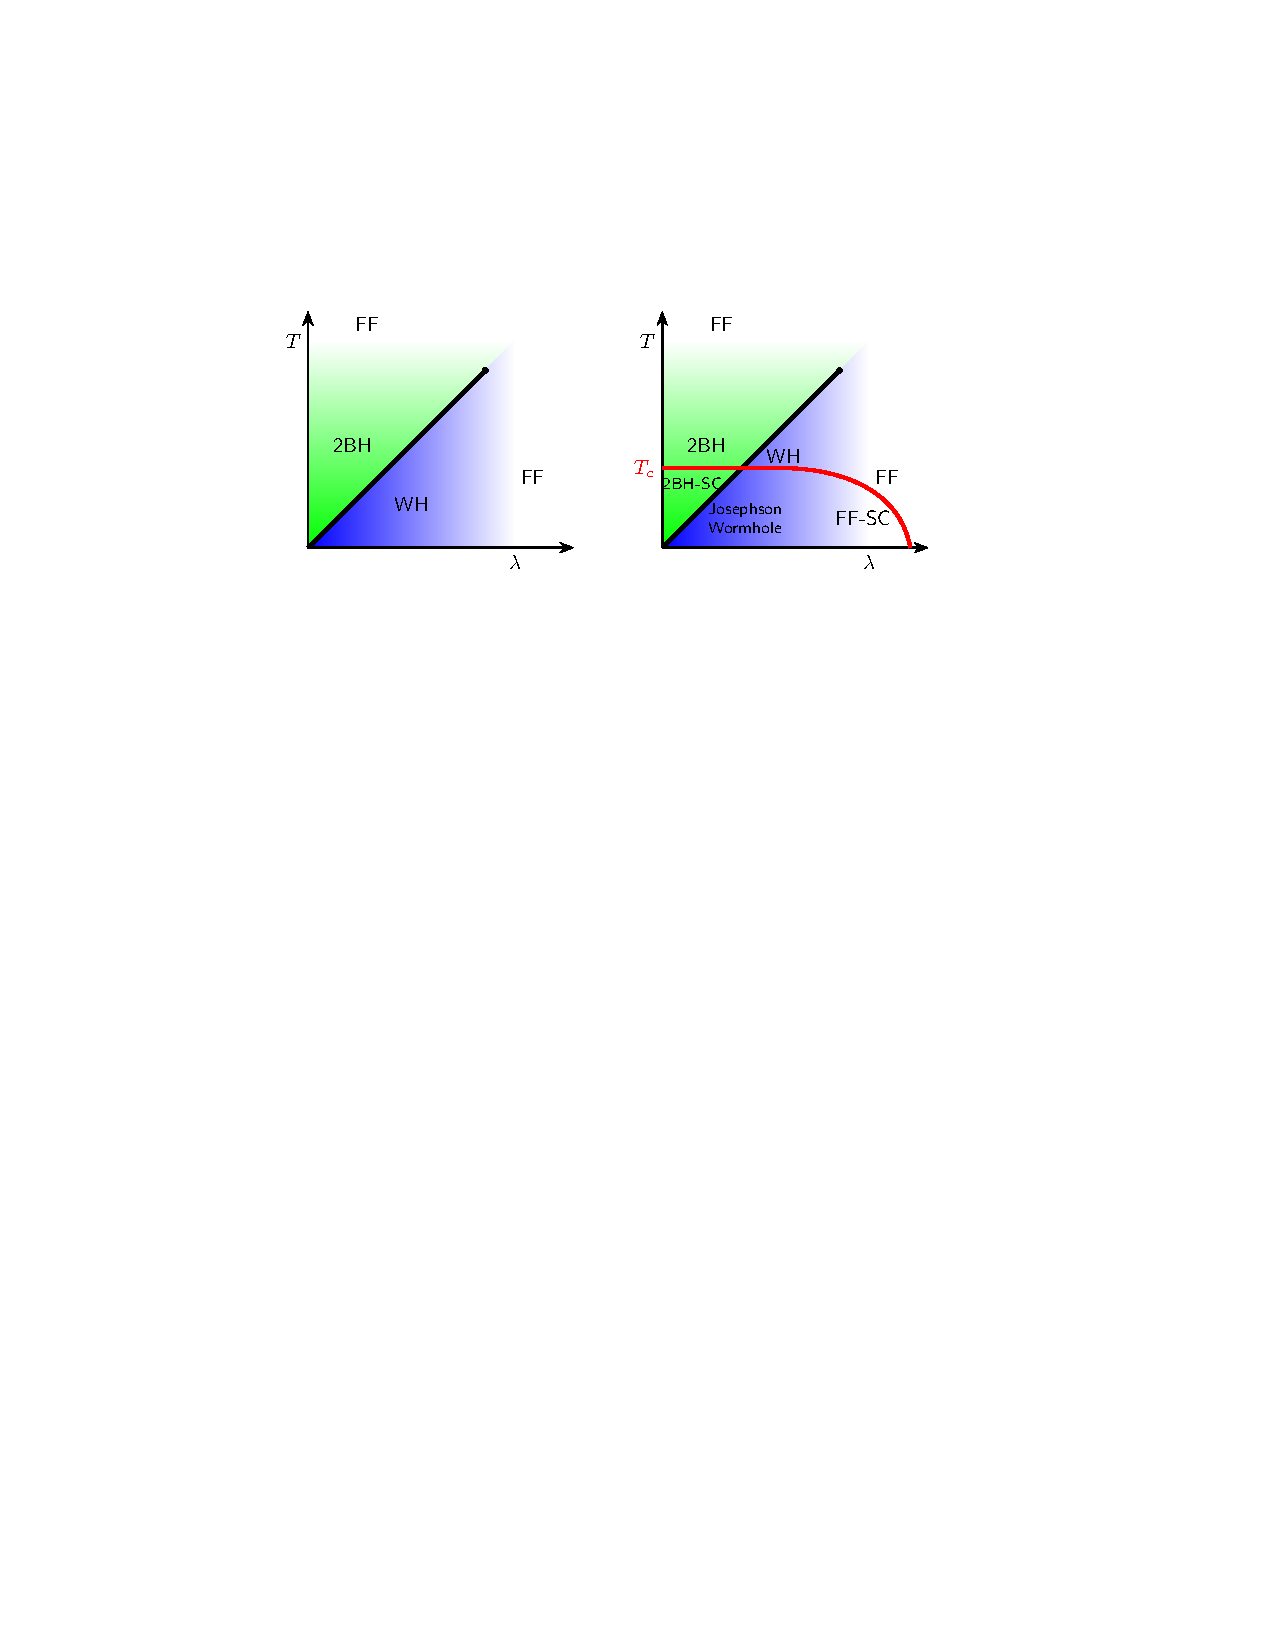
\includegraphics[width=0.9\linewidth]{2YSYK-PhaseDiagram.pdf}
    \caption{
        Schematic Phase diagram in the non-superconducting state. We find two kinds of free fermion phases that are smoothly connected to each other. On lowering the temperature, we find first powerlaw correlations developing in the diagonal green's function. We call this non-fermi liquid state (NFL) which is dual to a two sided black hole geometry. At the lowest temperatures however, i.e. when $T \ll \lambda $, the system undergoes a first order transition to the wormhole state. The two phases are demarcated by a line $T \sim \lambda$}
    \label{fig:Schematic Phase diagram}
\end{figure}

\begin{itemize}
    \item {\bf Characteristics}
    \item Anomalous scaling of fermion and phonon Green's functions and order parameter.
    \item Ordered of lowest lying states
    \item Josephson current
    \comment{DC Josephson current $I_c$ is related to the superconducting gap (Ambegaokar-Baratoff- relation). What happens here? It is also related to the superfluid density. What happens for the pairing revival (four point function?)/Numerics}
    \item 
\end{itemize}





%##################

\section{Two Y-SYK models with a tunneling contact.}
\label{sec:model}

\noindent
The model represents two quantum dots that contain $2N$ flavors of fermions (including spin) and $M$ flavors of bosons on each of them respectively, and described separately by the Yukawa SYK Hamiltonian, with exactly the same realization of disorder on each side. We are interested in this model in the of large fermion and boson flavors $M\rightarrow\infty$, $N\rightarrow\infty$, such that the ratio $\kappa = \nicefrac{M}{N}$ is constant.
\begin{widetext}
\begin{equation}
    H_{Y-SYK} = -\mu\sum_{i=1}^N\sum_\sigma c^\dagger_{i,\sigma} c^{\phantom{\dagger}}_{i, \sigma} + \sum_{k=1}^M \frac{1}{2}\left(\pi_k^2 + \omega_0^2\phi_k^2\right) + \frac{\sqrt{2}}{N}\sum_{i,j,k}\sum_{\sigma}g_{ijk} c^\dagger_{i,\sigma} c^{\phantom{\dagger}}_{j,\sigma} \phi^{\phantom{\dagger}}_k
    \label{eq:HYSYK}
\end{equation}
\end{widetext}
This hamiltonian has a rich phase diagram showing non-Fermi liquid (NFL) physics at low temperature, described in Refs.~\cite{esterlis2019cooper,wang2020solvable,classen2021superconductivity}.

The two individual dots are then coupled by a fermion interaction across the two dots, of strength $\lambda$. The model is then described by the following action
\begin{widetext}    
\begin{align}
    S &= \left[\sum_{a=1,2} S^{(a)}_0 + S^{(a)}_{int}\right] + S_c \, , \nonumber \\
    S^{(a)}_{0} &= \int d\tau \sum_{i,\sigma} {c^\dagger}^{(a)}_{i\sigma}(\tau) \left(\partial_\tau - \mu\right)c^{(a)}_{i\sigma}(\tau) + \sum_k \phi^{(a)}_k(\tau)\frac{1}{2}\left(-\partial_\tau^2 + \omega_0^2\right) \phi^{(a)}_k(\tau) \, ,\nonumber\\
    S^{(a)}_{int} &= \frac{\sqrt{2}}{N}\int d\tau \sum_{ijk}\sum_{\sigma}  g_{ijk}{c^\dagger}^{(a)}_{i\sigma}(\tau)c^{(a)}_{j\sigma}(\tau)\phi^{(a)}_k(\tau) \, ,\nonumber\\
    S_c &= \int d\tau \sum_{i,\sigma}\lambda {c^\dagger}^{(1)}_{i\sigma}(\tau)c^{(2)}_{i\sigma}(\tau) + \lambda^* {c^\dagger}^{(2)}_{i\sigma}(\tau)c^{(1)}_{i\sigma}(\tau) + \sum_k J\phi^{(1)}_k(\tau)\phi^{(2)}_k(\tau) \,.
    \label{eq:bareaction}
\end{align}
\end{widetext}
In what follows, we will refer to the two dots with indices $(1,2)$ or $(L,R)$ respectively, and refer to the system as the two-sided Yukawa SYK model. 

The $g_{ijk}$ are in general random complex numbers, but they are all not independent, and have constraints imposed by requiring that the hamiltonian be hermitian. In the absence of time-reversal symmetry (TRS), the couplings $g_{ijk}$ would be drawn from the Gaussian Unitary ensemble (GUE). When TRS is present however, the couplings would need to be drawn from the Gaussian Unitary ensemble (GUE). 

In the rest of the article, we will work with $g=0.5$ and at the charge neutrality point $\mu=0$. These parameters are chosen so that the finite temperature state of the one-sided model exhibits only the NFL phase and not the impurity phase~\cite{esterlis2019cooper}. For convenience, we will also set $J=0$ and study the model only with the bare fermion cross coupling $\lambda$ explicitly introduced. It can be noted that a coupling between the bosons on the two sides will be dynamically generated through a fermion mediated mechanism.

This model can be expressed in terms of the $G-\Sigma$ theory by integrating out all the fermions and bosons, and one can obtain the saddle point solutions to the Euler-Lagrange equations. Details of the derivation are given in the appendix~\ref{app:effectiveaction}. 
$G_{ab}(\tau,\taup)$ now stands for $-\frac{1}{N} \sum_i\cind{a}{i}{\tau}\cdag{b}{i}{\taup}$. 


%#
\section{Description of the metallic state}
\label{sec:metallic-state}
%
Since the two sided action in appendix~\ref{app:effectiveaction} explicitly couples the different copies, one cannot impose a replica symmetric action as is usually done in the SYK literature. However, an additional symmetry can be used to reduce the number of Green's functions one needs to keep in the computations. 
We observe symmetry upon swapping the two layers. 
\begin{align}
    c_1 &\rightarrow c_2 e^{i\theta}\\
    c_2 &\rightarrow c_1 e^{-i\theta} \\
    \phi_1 &\leftrightarrow \phi_2  
    \label{eq:mirror_symmetry}
\end{align}
leaves the action invariant: this is the definition of mirror symmetry for this case. The point is that no matter what phase the complex coupling $\lambda$ has, we can pick $\theta$ appropriately for the symmetry to hold. Thus, we can make a gauge choice $\lambda$ to be purely real, giving $\theta = 0$. This leaves, $G_{11}=G_{22}=G_d$ and $G_{12} = G_{21} = G_{od}$. This is the convention we will stick to in what follows. As a side remark, notice that if we had picked as a gauge choice $\lambda$ to be purely imaginary, we would have had $G_{11} = G_{22}$ and $G_{12} = -G_{21}$. 
%
This leaves us with the Schwinger-Dyson equations: 
\begin{align}
    \det G &= (i\omega_n + \mu -\Sigma_d)^2 - (\lambda - \Sigma_{od})^2 \\
    G_d(i\omega_n) &= \frac{i\omega_n + \mu -\Sigma_d}{\det G}\\ 
    G_{od}(i\omega_n) &= -\frac{(\lambda - \Sigma_{od})}{\det G} \\
    \det D &= (\nu_m^2 + r - \Pi_d)^2 - (J - \Pi_{od})^2 \\
    D_d(i\nu_m) &= \frac{\nu_m^2 + r - \Pi_d(i\nu_m)}{\det D} \\
    D_{od}(i\nu_m) &= -\frac{(J - \Pi_{od})}{\det D}\\
    \Sigma_{(o)d}(\tau) &= \kappa g^2\, D_{(o)d}(\tau) G_{(o)d}(\tau)\\
    \Pi_{(o)d}(\tau) &= -2 g^2\, G_{(o)d}(\tau)G_{(o)d}(-\tau)
    \label{eq:SDeqnsmetal}
\end{align}
%
The self energies remain the same as for the single side case for both the diagonal and off diagonal components. These equations can be solved numerically in imaginary time and Matsubara frequency and their results are shown in Fig.~\ref{fig:GreenFunctionPlotsMetal}.
%
\subsection{Free fermion phases}
From dimensional analysis, the SYK coupling can be expected to be important at an energy scale of $T_{SYK} \sim g^{\nicefrac{2}{3}}$. 
The phase diagram of the non-superconducting state in the $T-\lambda$ plane contains two free fermion limits, when the scale $T_{SYK}$ is not the dominant one as is represented in Fig.~\ref{fig:Schematic Phase diagram}. 
%
The high temperature phase, when $\nicefrac{T}{\lambda} \gg 1 $, the system is the free fermion phase FF1, and the diagonal Green's function is well approximated by $G_{d}(\tau)\sim -\frac{1}{2}\sgn(\tau)$. Correspondingly, $G_{d}(i\omega_n) \sim \frac{1}{i\omega_n} $. This represents the situation in which the fermions are separately free in each dot.
%
The other free fermion phase FF2 is seen when $\nicefrac{T}{\lambda}\ll 1$ and $\lambda, T \gg T_{SYK}$ the diagonal Green's function is well approximated by turning off the self-energies in Eq.~\eqref{eq:SDeqnsmetal} and taking the limit of zero temperature, so that 
\begin{align}
    G_d^0(\tau) &= \int_{-\infty}^{\infty} \frac{d\omega}{2\pi}\, \frac{i\omega}{(i\omega)^2 - \lambda^2} \nonumber \\
    &= -\frac{1}{2}\sgn(\tau) e^{-\lambda\abs{\tau}}.
    \label{eq:Gd0taulambda}
\end{align}
This represents a situation when the fermions just occupy the ground state of the cross coupling part of the hamiltonian, but are otherwise free. When analytically continued to the real axis, the spectral function would simply represent a quasiparticle pole at $\pm\lambda$.
%
The two phases FF1 and FF2 are smoothly deformable to each other, and indeed the FF2 form of the diagonal Green's function becomes the FF1 form in the limit of $\lambda\rightarrow 0$.
%
\subsection{Interacting fermion phases}
Upon starting from the high temperature phase FF1 and lowering temperature below the scale $T_{SYK}$, we see the onset of the NFL state and its emergent conformal symmetry. At low frequencies, the diagonal Green's functions scale with a power law 
\begin{align}
    G(\omega) &\sim \abs{\omega}^{2\Delta_f-1}\sgn(\omega) \\
    D(\omega) &\sim \abs{\omega}^{2\Delta_b-1} \,.
    \label{eq:scalingsolns}
\end{align}
In these equations, $\Delta_f$ and $\Delta_b$ are the scaling dimensions of the fermions and bosons respectively, and can be calculated in the conformal limit of the Schwinger-Dyson equations. They need to satisfy
\begin{align}
    2\Delta_f + \Delta_b &= 1 \, ,\\
    \kappa\frac{\Gamma(1-\Delta_f)\Gamma(1-(\Delta_f+\Delta_b))}{\Gamma(\frac{1}{2}+\Delta_f)\Gamma(\frac{1}{2}+\Delta_f+\Delta_b)} &= -2 \frac{\Gamma(\frac{1}{2}-\Delta_b)\Gamma(\frac{1}{2}-2\Delta_f)}{\Gamma(\Delta_b)\Gamma(2\Delta_f)} .
\end{align}
%
\begin{figure}[h]
    \centering
    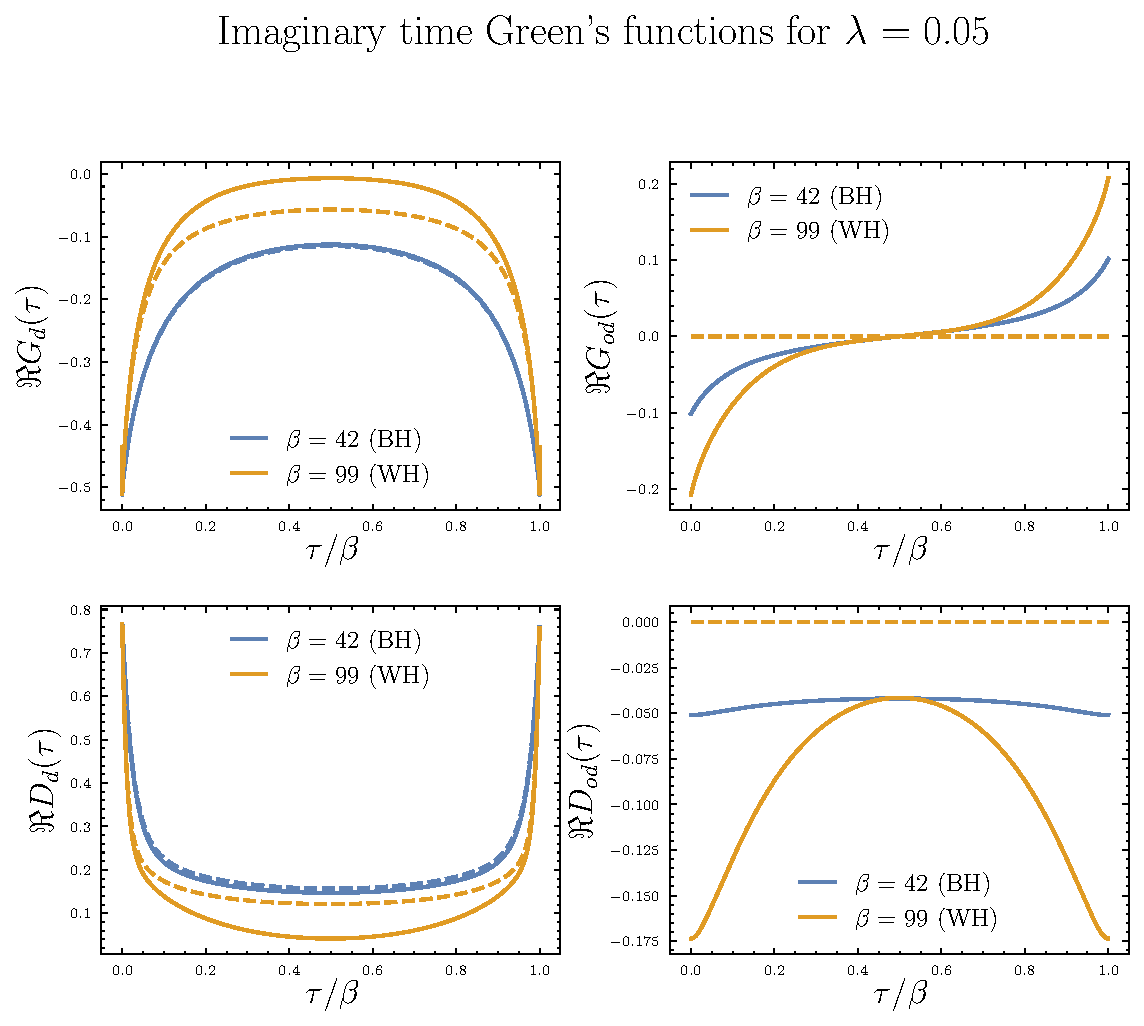
\includegraphics[width=\linewidth]{GreenFunctionPlotsMetal.pdf}
    \caption{Imaginary time Green's functions at on lowering temperature at fixed $\lambda$ in the metallic state. The dotted lines show an analytic approximation for the one sided Yukawa SYK model from Ref.~\cite{esterlis2019cooper} at the corresponding temperature. These figures indicate that in the wormhole phase, off-diagonal correlations are enhanced and diagonal correlations are suppressed.}
    \label{fig:GreenFunctionPlotsMetal}
\end{figure}

Fig.~\ref{fig:GreenFunctionPlotsMetal} for $\beta=50$ shows the numerically exact solutions to the Schwinger-Dyson equations for this case. At short time, the Green's functions decay by a power law $G_d(\tau) \sim \frac{1}{\abs{\tau}^{2\Delta_f}}$ and $D_d(\tau) \sim \frac{1}{\abs{\tau}^{2\Delta_b}}$. 
On the gravity side, this power-law correlated state represents the two-sided black hole (2BH) geometry, and is the red region in the phase diagram Fig.\ref{fig:Schematic Phase diagram}.
%
On further lowering temperature, the state with power law correlations jump over into a state with exponentially decaying correlations as a first order phase transition. This is the $\beta=80$ curve in Fig.~\ref{fig:GreenFunctionPlotsMetal}. This solution could also be obtained alternatively in a smooth manner by starting from the state FF2 at large $\lambda$ described above, and then reducing $\lambda$ below the scale $T_{SYK}$. 
In this case, the diagonal Green's functions are faithfully represented by the form 
\begin{align}
    G_d(\tau) \sim e^{-\gamma \tau}. 
\end{align}
Unlike the free-fermion state FF2, for which $\gamma = \lambda$, the exponent varies as a function of $\lambda$ as is varied at a constant temperature. It was predicted in Ref.~\cite{maldacena2018eternal} that the gap should scale as 
\begin{align}
    \gamma[\lambda] \sim \lambda^{\frac{1}{2-2\Delta}}. 
    \label{eq:gapscaling}
\end{align}
For the complex SYK model with $\Delta=\frac{1}{4}$, this exponent is $\gamma[\lambda] \sim \lambda^{\nicefrac{2}{3}}$. and was observed numerically in Refs.~\cite{maldacena2018eternal,qi2020coupled,sahoo2020traversable}. 
%
For the two sided Yukawa-SYK model that we consider presently, since we couple only the fermions across the two sides, we can confirm from dimensional analysis that both the boson and fermion Green's functions should scale exactly as in Eq.~\eqref{eq:gapscaling}, with $\Delta = \Delta_f$. Our results showing this scaling is represented in Fig. ~\ref{fig:ImagTimeScaling}. Starting from the numerical solutions to Eqs.~\ref{eq:SDeqnsmetal}, we obtain mass gap from the logarithmic derivative of $G_d(\tau)$ and $D_d(\tau)$ in the long time regime where we expect the exponential decay and then fit how it changes with lambda. We observe strong agreement between the dimensional analysis result and the numerical computation.  
%
On the gravitational side, this state with exponentially decaying correlations that scale in the manner of Eq.~\eqref{eq:gapscaling} represent an eternal traversable wormhole(WH) geometry. 
%
\begin{figure}[h]
    \centering
    \begin{subfigure}[t]{0.2\textwidth}
        \centering
        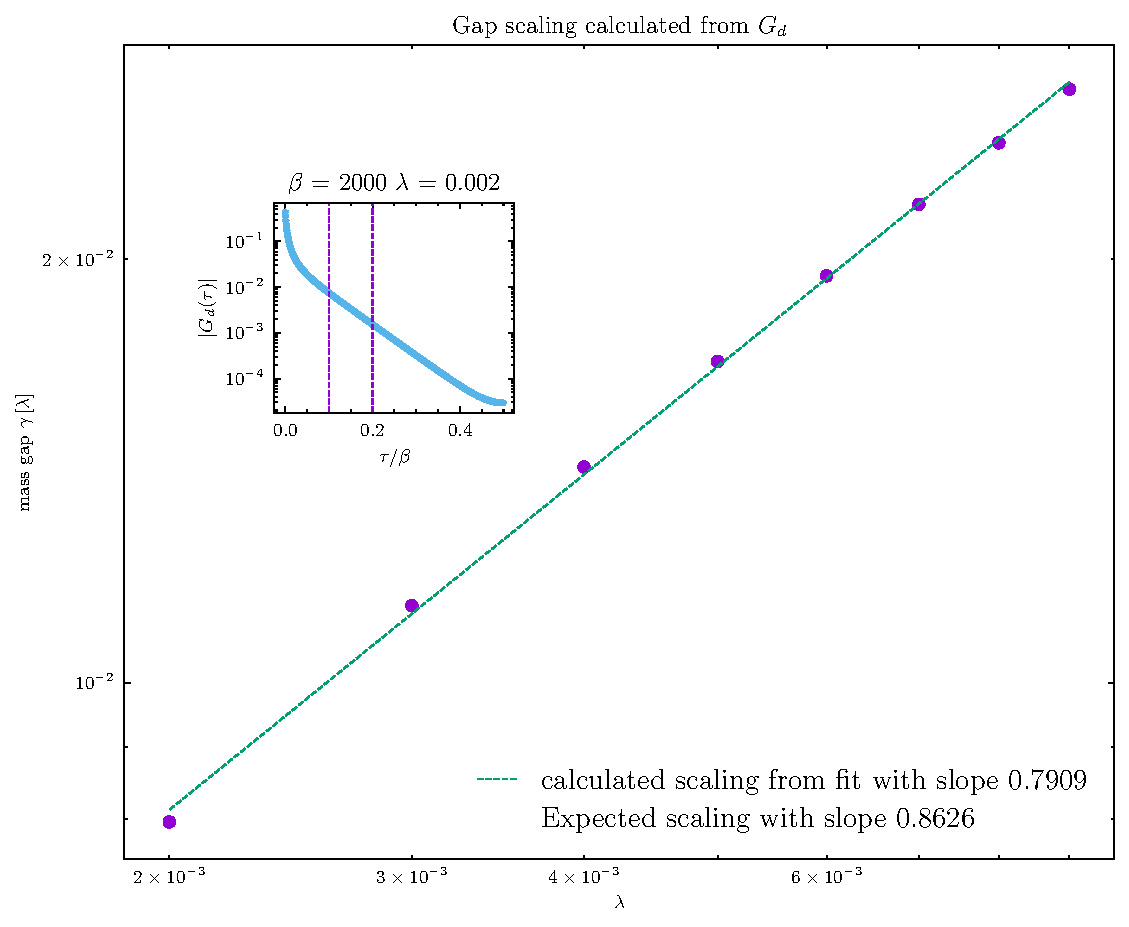
\includegraphics[width=\textwidth]{GdGapscaling.pdf}
        \caption{}
        \label{fig:ImagTimeGapscalingGkappa1}
    \end{subfigure}
    ~\begin{subfigure}[t]{0.2\textwidth}
        \centering
        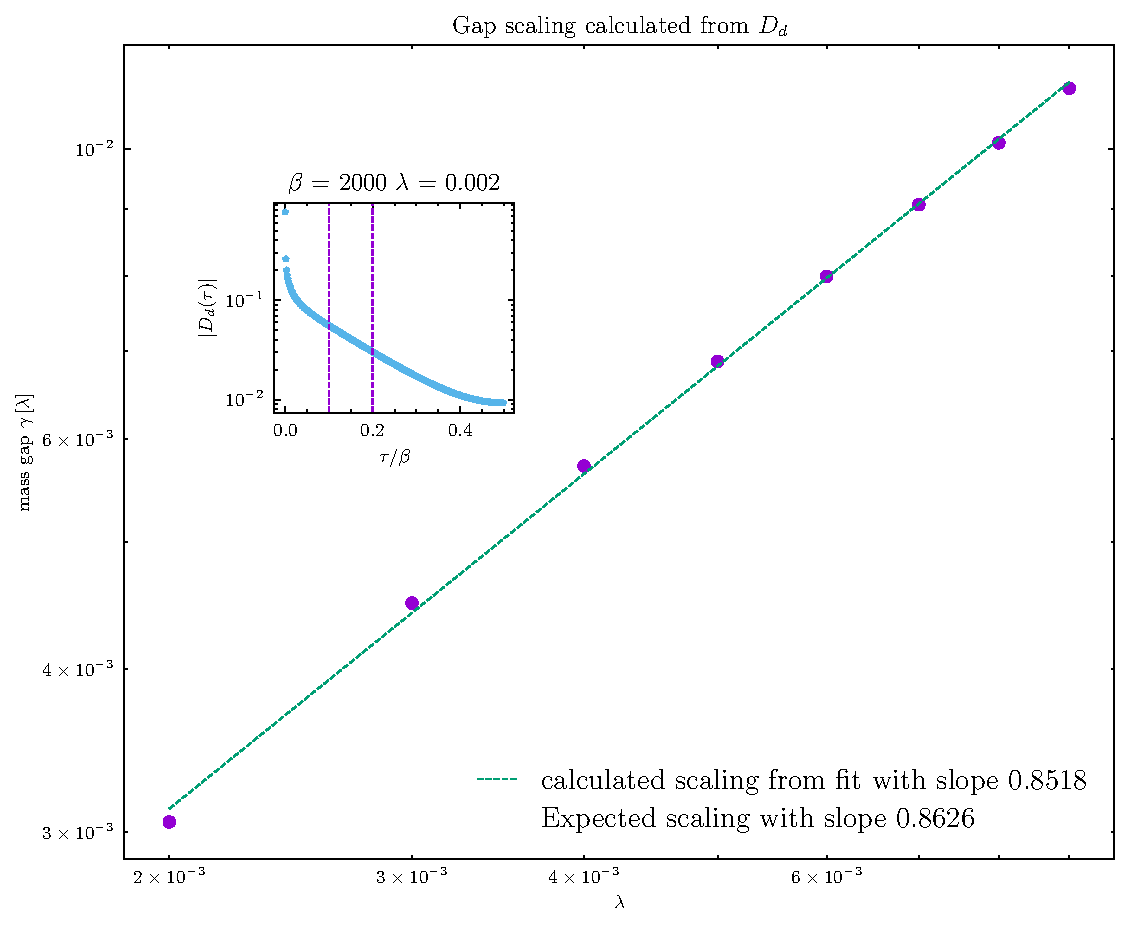
\includegraphics[width=\textwidth]{DdGapscaling.pdf}
        \caption{}
        \label{ImagTimeGapscalingDkappa1}
    \end{subfigure}
    ~\begin{subfigure}[t]{0.2\textwidth}
        \centering
        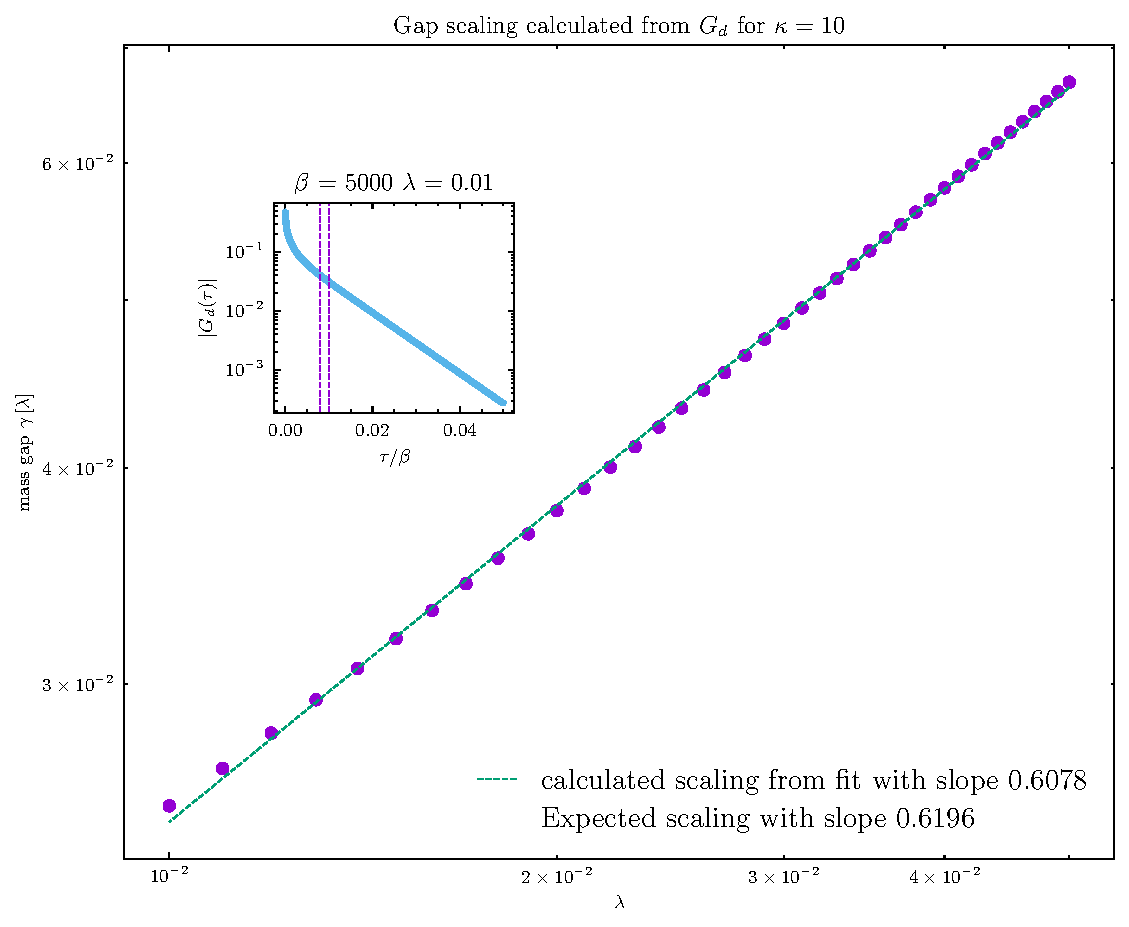
\includegraphics[width=\textwidth]{kappa10GdGapscaling.pdf}
        \caption{}
        \label{fig:ImagTimeGapscalingGkappa10}
    \end{subfigure}
    ~\begin{subfigure}[t]{0.2\textwidth}
        \centering
        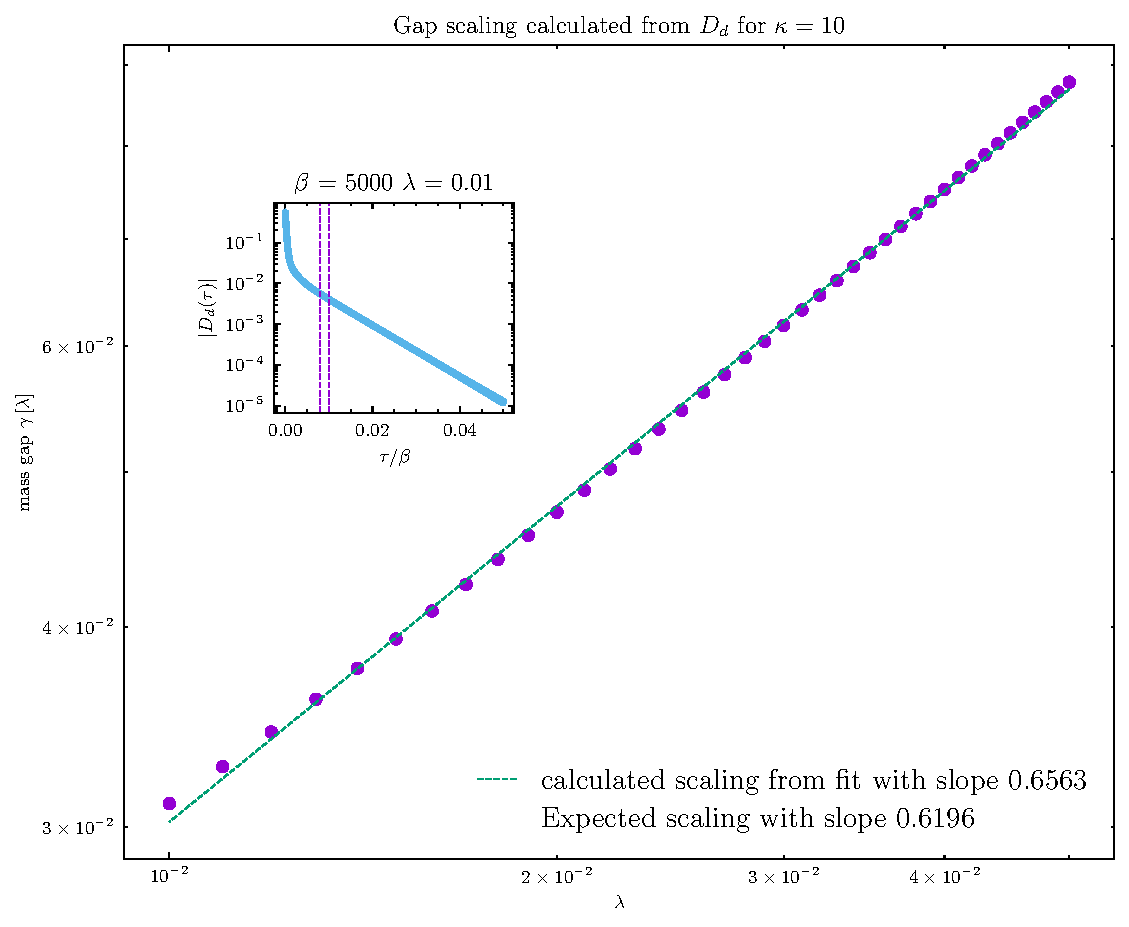
\includegraphics[width=\textwidth]{kappa10DdGapscaling.pdf}
        \caption{}
        \label{ImagTimeGapscalingDkappa10}
    \end{subfigure}
    \caption{Scaling of the gap with the cross coupling $\lambda$. Panels(a) and (b) show the diagonal fermion and boson green's function respectively for $\kappa$ = 1 and $\Delta = 0.42$ respectively. Panels (c) and (d) show the same scaling upon changing the effective slope by increasing $\kappa$ to 10, and hence reducing $\Delta$ to $0.193$. There is good agreement between the expected $\lambda^{\frac{1}{2-2\Delta}}$ scaling based on dimension analysis to the exact numerical solution. The insets show the exponential behavior of the respective Green's functions, and the window marked with the purple dotted lines indicate the region where the fit was performed for each data point of the main panels.}
    \label{fig:ImagTimeScaling}
\end{figure}
%
\subsection{Spectral functions in the wormhole state}
Using standard SYK tricks, we can numerically perform the analytical continuation to real frequencies to obtain the retarded correlators and the spectral functions in the 2BH and WH states. 
Their temperature evolution is depicted in Fig.~\ref{fig:GreenFunctionPlotsMetalv1} and ~\ref{fig:GreenFunctionPlotsMetalv2}. 
%
For the fermions, in the NFL or 2BH state, the spectral function is akin to the single Yukawa-SYK case with a single peak at zero frequency, and a power law decay. As temperature is lowered below the wormhole transition temperature, the central peak splits into two. These peaks are not placed at $\pm \lambda$, like they would be in the FF2 limit. Indeed these peaks have a weak temperature dependence, and upon cooling even deeper into the phase, the peaks move further away from $\omega = \lambda$. This is starkly noticeable especially in Fig.~\ref{fig:GreenFunctionPlotsMetalv1}. 
%
In our study we did not notice any higher peaks similar to the tower of conformal states seen for example in Ref.~\cite{plugge2020revival,sahoo2020traversable,qi2020coupled} for the majorana and complex SYK models. This could possibly be attributed to the higher peaks being spaced too far away in frequency, but this remains to be investigated. 
%
\begin{figure}[h]
    \centering
    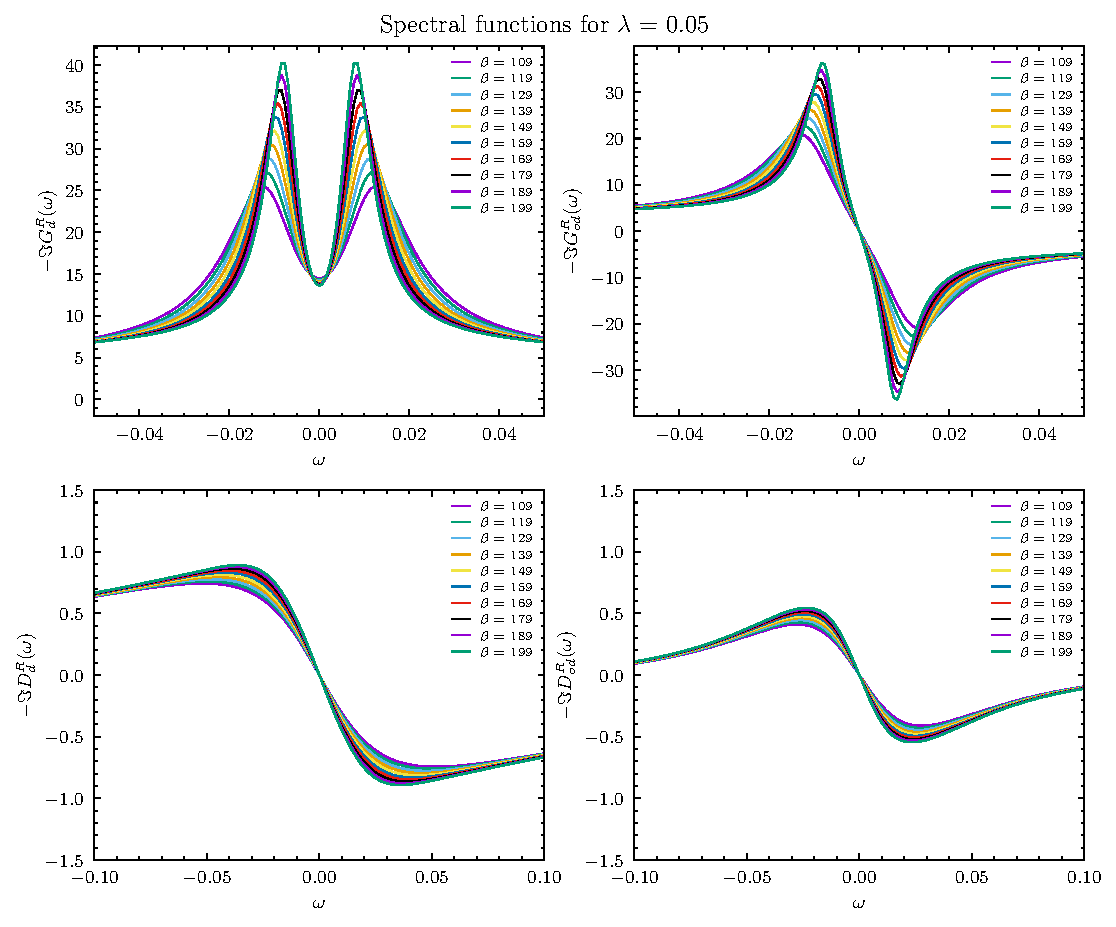
\includegraphics[width=\linewidth]{v1TempEvolnSpectralGapMetalWH.pdf}
    \caption{Temperature evolution of wormhole spectral function. The wormhole state is characterized by a single split peak, and the tower of conformal states is not observed in our numerics. This can be compared to the spectral function in the large $q-$ limit of study of Qi and Zhang (Ref.~\cite{qi2020coupled}).}
    \label{fig:GreenFunctionPlotsMetalv1}
\end{figure}

\begin{figure}[h]
    \centering
    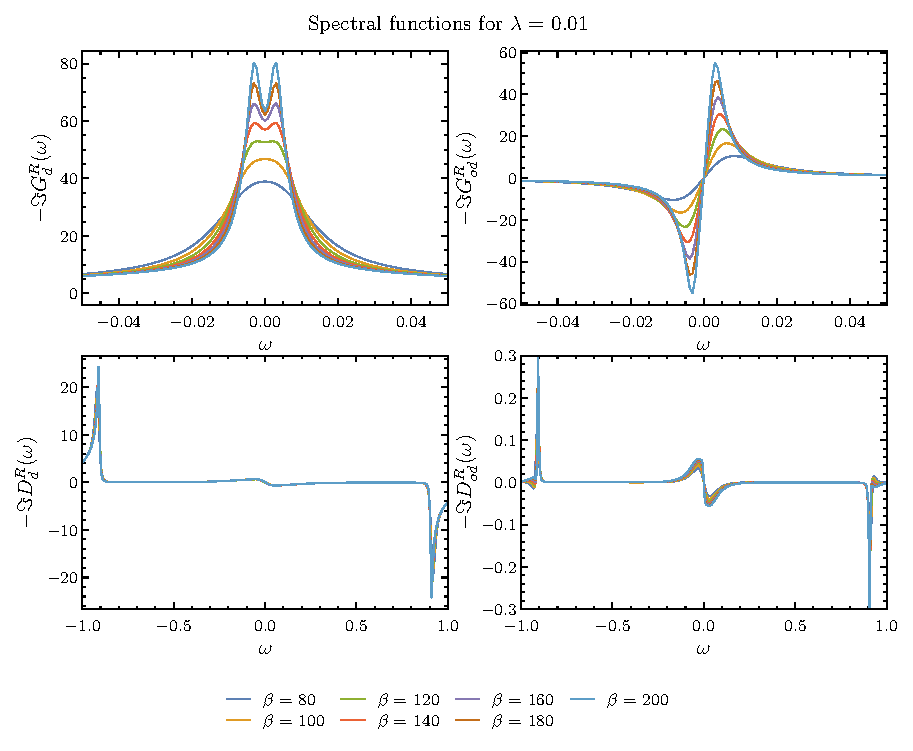
\includegraphics[width=\linewidth]{v3TempEvolnSpectralGapMetalWH.pdf}
    \caption{\textbf{ALTERNATE CHOICE OF FIGURE}Temperature evolution of coupled spectral function. The wormhole state is characterized by two symmetrically placed split peaks, but the black hole state is characterized by a smooth spectral function with the NFL form. This can be compared to the spectral function in the large $q$- limit of study of Qi and Zhang (Ref.~\cite{qi2020coupled}).}
    \label{fig:GreenFunctionPlotsMetalv2}
\end{figure}



%#
\newpage
\section{Inclusion of superconductivity}
\label{sec:sc-state}
We start from the disorder averaged action with the imposed spin-singlet constraints sketched in appendix~\ref{app:effectiveaction}.  
We first look at the case when $\lambda$ is a real coupling. In this case, both sides are identical to one another, and we also expect the superconducting state to be mirror symmetric under the mirror symmetry in Eq.~\eqref{eq:mirror_symmetry}. 
%
In the saddle point equations, we can then also additionally impose $F_{11} = F_{22} = F_{d}$ and $F_{12} = F_{21} = F_{od}$, and likewise for the self energies. 
%
\begin{figure}[h!]
    \centering
    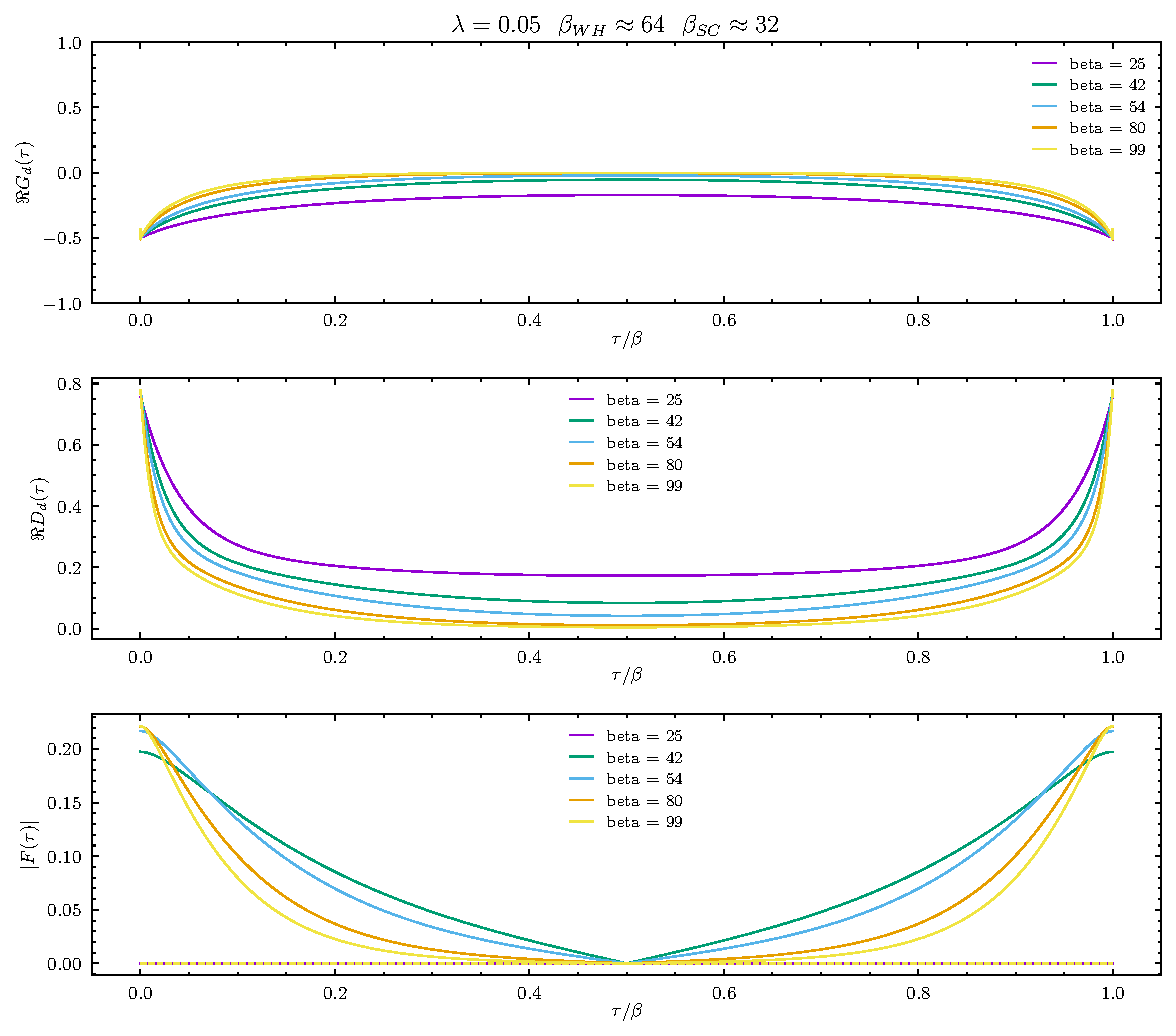
\includegraphics[width=0.5\linewidth]{SupCondLinear.pdf}
    \caption{Superconducting solutions to the Two sided model. In the bottom panel, dotted lines indicate the off diagonal anomalous propagator $F_{od}$.}
    \label{fig:SuperconductingGFsImagTime}
\end{figure}
Fig.~\ref{fig:SuperconductingGFsImagTime} shows the exact numerical solution to the saddle point equations including the presence of the anomalous propagator terms. 
%
At the highest temperatures, the system free fermion system is non-superconducting, as indicated by the vanishing anomalous propagators. As the temperature is lowered, it enters the metallic 2BH state with its power law correlation in the fermionic single particle Green's functions. Shortly in this phase, upon only gently lowering the temperature, the system starts superconducting, as evidenced by the superconducting order parameter $\Delta(i\omega_n) \rightarrow 0)  $ or alternatively $F_{d}(\tau = 0^{+}) $ attaining a finite expectation value. Upon further lowering the temperature into the wormhole state, its superconductivity is maintained.
%
In both superconducting phases, we observe a striking similarity in the nature of the formed cooper pairs. Numerically, we observe that when superconductivity wins over, the off diagonal terms of the anomalous propagator $F_{12}$ and $F_{21}$ are still vanishingly small, and the diagonal terms $F_{11}$ and $F_{22}$ are the ones that take on a non-zero expectation value (Fig.~\ref{fig:MagnitudeSelfEnergies}). This indicates that the cooper pairs are still well formed separately on either side. 
%
\begin{figure}[h]
    \centering
    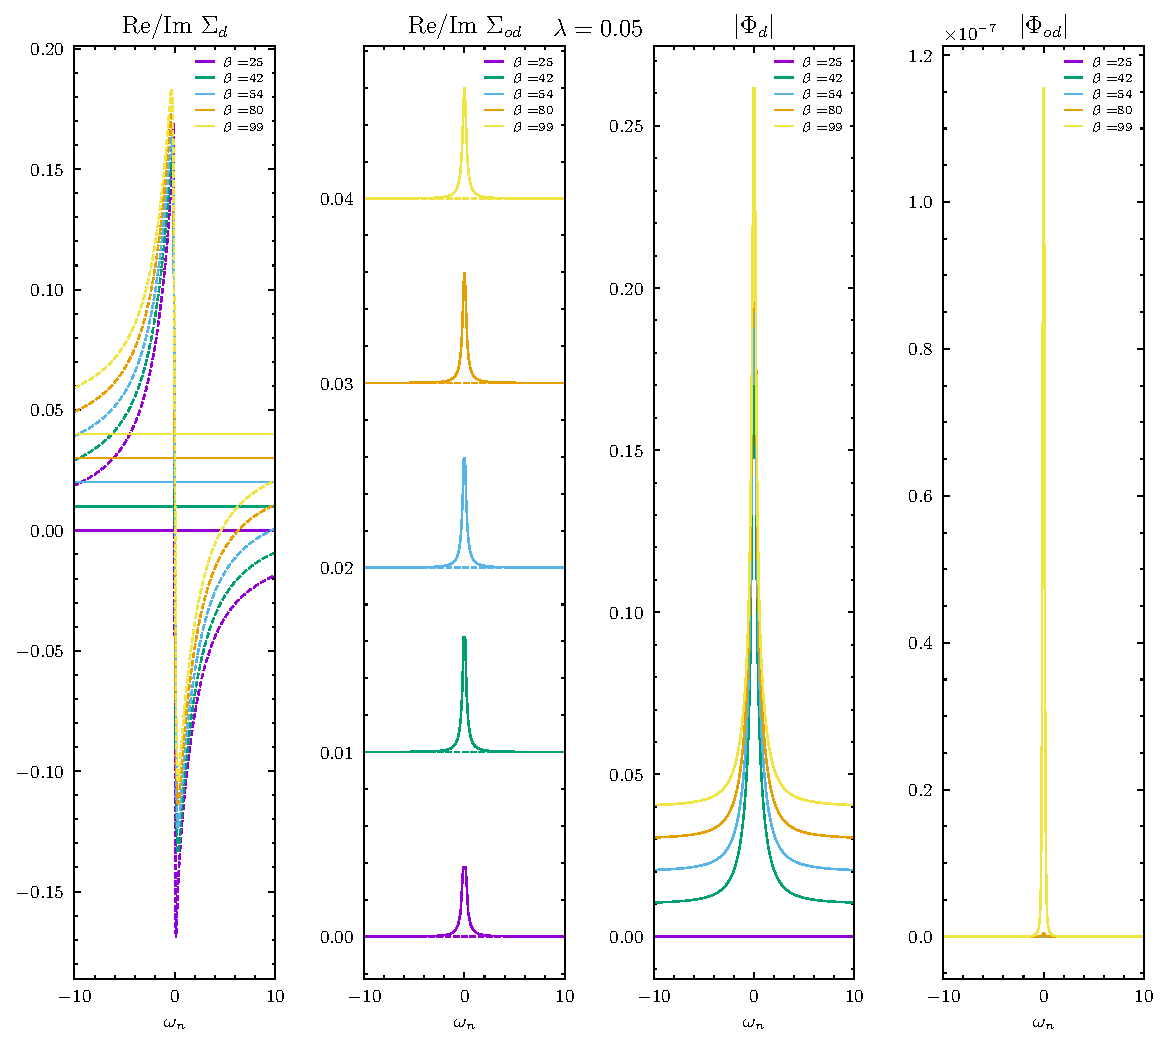
\includegraphics[width=0.5\linewidth]{Magnitude of self energies.pdf}
    \caption{Magnitude of the various self energies in the superconducting state. In the first two panels, the solid lines indicate the real parts and the dotted lines indicate the imaginary parts. The different curves have been manually offset for ease of presentation.}
    \label{fig:MagnitudeSelfEnergies}
\end{figure}
The vanishing of the off-diagonal superconducting correlations can be understood in the following way. In the large $\lambda$ limit, the metallic state is composed of a trivial singlet state, which is gapped out. We also numerically verify that this state is not superconducting even until the lowest temperatures we can reach. 
%
This evidence that the phase of the superconducting wave function is well defined on either side is indication that the phase may be twisted independently giving rise to a Josephson-like effect. 

\section{Josephson Current}
When a tunnel junction is formed by separating a superconducting ring with a weak link, the threading of magnetic flux through it can be understood as the phase of the hopping parameter connecting the two sides of the junction. The coupling term in Eq.~\eqref{eq:bareaction} is then
\begin{align}
    S_c &= \abs{\lambda}\left[e^{i\theta} c_1^\dagger c_2^{\phantom{\dagger}} + e^{-i\theta} c_2^\dagger c_1^{\phantom{\dagger}}\right] \nonumber \\
    &= \abs{\lambda}\left[c_1^\dagger \tilde{c}_2^{\phantom{\dagger}} +  \tilde{c}_2^\dagger c_1^{\phantom{\dagger}}\right] 
    \label{eq:transphasetocops}
\end{align}

Alternatively, the phase of the coupling $\lambda$ can be reabsorbed into one of the fermions by refining $\tilde{c}_2 = c_2 \,e^{i\theta}$. In the new variables $c_1, \tilde{c_2}$, the action is identical as the case with real $\lambda$, and the rotated phase $\theta$ in the physical pair of variables $c_1, c_2$ appears through the saddle point constraints in the Green's functions and their self energies.
This is first illustrated in the BCS limit in the following section. 
\subsection{BCS limit of the Josephson current}
In the BCS limit of two superconductors coupled by a weak link, the two sided hamiltonian can be written down as~\cite{tummuru2022josephson}
\begin{align}
    H &= \left(
    \begin{array}{cccc}
     \xi  & \Delta  & t & 0 \\
     \Delta  & -\xi  & 0 & -t \\
     t & 0 & \xi  & \Delta  e^{2 i \theta } \\
     0 & -t & \Delta  e^{-2 i \theta } & -\xi  \\
    \end{array}
    \right), 
\end{align}
where the absorbed phase of $\theta$ appears as a phase difference of $2\theta$ between superconducting order parameters of the two sides. It can be noted in this case that this is the term that is $\theta$ dependent and the rest of the entries are gauge invariant.
%
The green's functions of this model are simply expressed by 
\begin{equation} 
    G(i\omega_n) = \left(i\omega_n \mathbb{1} - H \right)^{-1}
\end{equation}
%
Then, the free energy can be written as (with $E^2 = \xi^2 + \Delta^2 $ by analogy)
\begin{align}
    \mathcal{F} &= -\sum_{\omega_n} \log\det\left(i\omega_n \mathbb{1} - H\right) \, , \nonumber\\
    &= -\log \left(\left(\Delta ^2+\xi ^2+\omega_n ^2\right)^2+t^4+2 t^2 \left(\Delta ^2 \cos (2 \theta )-\xi ^2+\omega_n ^2\right)\right) \, , \nonumber \\ 
    &= -\sum_{\omega_n} \log\left[(\omega_n^2 + E^2)^2 + t^4 + 2t^2(\omega_n^2-\xi^2) + 2t^2\Delta^2\cos(2\theta)\right] \, , \nonumber \\
    &= -\sum_{\omega_n}\log\left[f(\omega_n) + 2t^2\Delta^2\cos(2\theta)\right].
\end{align}
In the limit of a Josephson junction with a weak link, we can neglect higher order terms in the coupling $t$, and $f(\omega_n)$ is well approximated by simply $(\omega_n^2 + E^2)^2$. 
The Free energy can then be written in the form that is known from gauge rotation arguments in Ginzburg-Landau theory to be 
\begin{align}
    \mathcal{F} &= =\sum_{\omega_n} \log f(\omega_n) - \log\left(1+ \frac{2t^2\Delta^2\cos(2\theta)}{f(\omega_n)}\right) \, , \\
    &\approx \mathcal{F}_0 - \sum_{\omega_n} \frac{2t^2\Delta^2}{f(\omega_n)} \cos{2\theta}. 
    \label{eq:FEBCSbare}
\end{align}
The critical Josephson current can be easily read off from the prefactor of the $\theta$ dependent term. The constant term $\mathcal{F}_0$ can be fixed by regularization with the free propagators. 
%
In the weak coupling limit, Eq.~\eqref{eq:FEBCSbare} can be massaged into a much more recognizable form by noticing that $\eval{F(\omega_n)}_{\xi=0} = \frac{\Delta}{(i\omega_n)^2 - \Delta^2}$, to get 
\begin{align}
    I_J^c = t^2 \sum_{\omega_n} F^\ast(\omega_n) F(\omega_n) 
\end{align}
which is just the bubble diagram with anomalous propagators.
%
\subsection{Josephson wormhole}
In the double sided Yukawa SYK model, we can add a phase to the coupling term $\lambda$ and transfer the phase to the $c_2$ operator in analogy with Eq.~\eqref{eq:transphasetocops}. The theory then in terms of the new operators $c_1$ and $\tilde{c}_2$ is identical to the mirror symmetric superconducting state discussed in Sec.~\ref{sec:sc-state}. 
%
However, in terms of the physical $c_1$ and $c_2$, the action can be written as 
\begin{align}
    S_f = -\ln\det
    \left(
    \begin{array}{cccc}
     i \omega _n -\Sigma _d  & -\Phi _d & -\lambda -e^{-i \theta } \Sigma _{\text{od}} & -e^{i \theta } \Phi _{\text{od}} \\
     -\bar{\Phi} _{\text{d}} & i \omega_n -\tilde{\Sigma} _{\text{d}}  & -e^{-i \theta } \bar{\Phi} _{\text{od}} & \lambda -e^{i \theta } \tilde{\Sigma} _{\text{od}} \\
     -\lambda -e^{i \theta } \Sigma _{\text{od}} & -e^{i \theta } \Phi _{\text{od}} & i \omega_n-\Sigma _d  & -e^{2 i \theta } \Phi _d \\
     -e^{-i \theta } \bar{\Phi} _{\text{od}} & \lambda -e^{-i \theta } \tilde{\Sigma} _{\text{od}} & -e^{-2 i \theta } \bar{\Phi} _{\text{d}} & i \omega_n -\tilde{\Sigma} _{\text{d}} \\
    \end{array}
    \right)
\end{align}
This is the only term in the full two sided action that depends on the rotated phase, the other terms being explicitly gauge invariant, as is evident from inspecting Eq.~\eqref{eq:Sbeforesiding}. The Free energy can be written in this case as 
\begin{align}
    \mathcal{F}  = -\sum_{\omega_n}\ln\left( f_0(\Sigma,\lambda,\omega_n) + f_1(\Sigma,\lambda,\omega_n) \cos\theta + f_2(\Sigma,\lambda,\omega_n)\cos{2\theta}\right) \,,
    \label{eq:exactFEJosWH}
\end{align}
with 
\begin{align}
    f_1 &= 2 \lambda  \left(2 \Sigma _{\text{od}}\left(\left| \Phi _d\right| {}^2+\lambda ^2+\omega ^2\right)+\Sigma _{\text{od}} \left| \Sigma _{\text{od}}\right|
   {}^2+4 i \omega_n  \Sigma _d \Sigma _{\text{od}}-2 \Sigma _d^2 \Sigma _{\text{od}}+\Sigma _{\text{od}}^3\right) \, ,\\
   f_2 &= 2 \lambda ^2 \left(\left| \Phi _d\right| {}^2+\left| \Sigma _{\text{od}}\right| {}^2\right) \,
\end{align}
where we have also used that at the saddle point, $\Sigma_d$ is purely imaginary and $\Sigma_{od}$ is purely real, and have also dropped terms involving $\Phi_{od}$ as it is order of magnitudes smaller that the other self energies on the saddle point (see Fig.~\ref{fig:MagnitudeSelfEnergies}). 
The origin of the $\cos\theta$ term can be understood already from the metallic case. Unlike conventional systems, the replica symmetry breaking in coupled SYK models leaves non-vanishing $G_{12}$. This has its origin in the identical realization of disorder on either side. 

We have explicitly calculated Eq.~\eqref{eq:exactFEJosWH} and used its derivative to calculate the josephson current. The results are shown in Fig.~\ref{fig:JosephsonCurrent}. We see that the Josephson current is periodic not with a period of $2\pi$ as in a conventional weak link junction, but with a phase of $4\pi$, owing to the contribution coming from the $G_{od}$ terms being non-vanishing in our theory.
\begin{figure}[ht!]
    \centering
    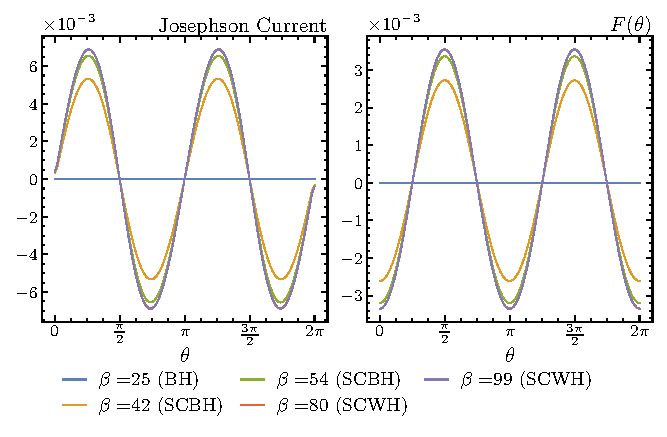
\includegraphics[width=0.5\linewidth]{JosephsonCurrent.pdf}
    \caption{DC Josephson current as a function of the phase angle. It should be noted that in this figure, the angle on the x-axis is the phase that was introduced on the complex hopping parameter $\lambda$, and the physical phase difference between the left and the right superconducting order parameters is $2\theta$. The non superconducting state also has a weak dependence of the  Inset: The corresponding free energy as calculated in Eq.~\eqref{eq:exactFEJosWH}, appropriately regulated, whose derivative with respect to the phase is shown in the main panel.}
    \label{fig:JosephsonCurrent}
\end{figure}






\section{Conclusion}
\label{sec:conclusion}

%##################
\begin{acknowledgments}
\noindent
We thank L. Barbera, N. Doerfler, I. Jang and J. Schmalian for discussions, and especially D. Valentinis and N. Chagnet both for discussions and help with the numerics. 
%We also thank  
This research was supported in part by the Dutch Research Council (NWO) project 680-91-116 ({\em Planckian Dissipation and Quantum Thermalisation: From Black Hole Answers to Strange Metal Questions.}), and by the Dutch Research Council/Ministry of Education.
%K.G. acknowledges funding from the European Union’s Horizon 2020 research and innovation programme under the Marie Sk\l odowska-Curie grant agreement No 101024967. 
The numerical computations were carried out 
%on the Dutch national Cartesius and Snellius national
%supercomputing facilities with the support of the SURF Cooperative (project EINF-468, EINF-2777, EINF-6933) as well as 
in part on the ALICE-cluster of Leiden
University. We are grateful for their help.

\end{acknowledgments}
%##################
\appendix
\section{Derivation of the effective action}
\label{app:effectiveaction}
%
Starting from the bare action, we will obtain the disorder averaged theory by performing the average over the couplings $g_{ijk}$. As discussed in the main text, we are interested in both the TRS broken (GUE) and TRS preserving (GOE) states to study the metallic and superconducting states respectively. We will thus interpolate between the two with the $\alpha$ parameter, which can be thought of as a pair breaking term in the superconducting state. To a certain extent, this parameter can also be used to tune the superconducting transition temperature, details of which are discussed at length in~\cite{classen2021superconductivity}. 
%
We will use the following lemma to do the disorder average in the $\alpha$ interpolating ensemble (for Hermitian $O_{ijk} = O^\dagger_{jik}$, as the case is here)
\begin{equation}
    \overline{e^{-\sum_{ijk} g_{ijk}O_{ijk}}} = \exp{-\sum_{ijk}\left[-\frac{1}{4}(1-\frac{\alpha}{2})\Bar{g}^2\left(O_{ijk} + O^\dagger_{ijk}\right)^2 + \frac{1}{4}(\frac{\alpha}{2})\Bar{g}^2\left(O_{ijk} - O^\dagger_{ijk}\right)^2\right]} \, ,
    \label{eq:alphaensemble}
\end{equation}
$\alpha = 0$ is the GOE and $\alpha=1$ is the GUE.  
%
The required terms in Eq.~\eqref{eq:alphaensemble} for our model are
\begin{multline}
    \left(O_{ijk} \pm O^\dagger_{ijk}\right)^2 = \sum_{a,b}\sum_{\sigma\sigma^\prime}\int d\tau\int d\tau^\prime \phind{a}{k}{\tau}\phind{b}{k}{\tau^\prime}\left[\cdag{a}{i\sigma}{\tau}\cind{a}{j\sigma}{\tau}\pm \cdag{a}{j\sigma}{\tau}\cind{a}{i\sigma}{\tau}\right]\\\left[\cdag{b}{i\sigmap}{\tau^\prime}\cind{b}{j\sigmap}{\tau^\prime}\pm \cdag{b}{j\sigmap}{\tau^\prime}\cind{b}{i\sigmap}{\tau^\prime}\right] \, .
    \label{eq:OpmO+}
\end{multline}
%
At this point, the following insertions of identity can be used to formally rewrite the action in terms of the collective $G-\Sigma$ variables~\cite{inkof2022thesis,valentinis2023correlation}
%
\begin{subequations} 
\begin{align}
    \mathbb{1} &= \int\mathcal{D}G\mathcal{D}\Sigma\, e^{-\left[-NG^{ba}_{\sigmap\sigma}(\taup,\tau) + \sum_i\cdag{a}{i\sigma}{\tau}\cind{b}{i\sigmap}{\taup}\right]\Sigma^{ab}_{\sigma\sigmap}(\tau,\taup)} \,,\label{eq:LMGS}\\
    \mathbb{1} &= \int\mathcal{D}F\mathcal{D}\Bar{\Phi}\, e^{-\frac{1}{2}\left[-NF^{ba}_{\sigmap\sigma}(\taup,\tau) + \sum_i\cind{a}{i\sigma}{\tau}\cind{b}{i\sigmap}{\taup}\right]{\Bar{\Phi}}^{ab}_{\sigma\sigmap}(\tau,\taup)}\,,\label{eq:LMFPhib} \\
    \mathbb{1} &= \int\mathcal{D}\Bar{F}\mathcal{D}\Phi\, e^{-\frac{1}{2}\left[-N{\Bar{F}}^{ba}_{\sigmap\sigma}(\taup,\tau) + \sum_i\cdag{a}{i\sigma}{\tau}\cdag{b}{i\sigmap}{\taup}\right]{\Phi}^{ab}_{\sigma\sigmap}(\tau,\taup)} \,,\label{eq:LMFbPhi}\\
    \mathbb{1} &= \int\mathcal{D}D\mathcal{D}\Pi\, e^{-\frac{1}{2}\left[MD^{ba}(\taup,\tau) - \sum_k\phi_k^{(a)}(\tau)\phi^{(b)}_{k}(\taup)\right]\Pi^{ab}(\tau,\taup)} \,. \label{eq:LMDPi}
\end{align}
\end{subequations}
%
We can write the interaction part of the action 
\begin{widetext}
\begin{align}
    \overline{S}_g = M\bar{g}^2\sum_{ab}\sum_{\sigma,\sigmap}\int d\tau \int d\taup D^{ab}(\tau,\taup)\left[G^{ab}_{\sigma\sigmap}(\tau,\taup)G^{ba}_{\sigmap\sigma}(\taup,\tau) + (1-\alpha)\Bar{F}^{ab}_{\sigma\sigmap}(\tau,\taup)F^{ab}(\tau,\taup)\right] 
\end{align}
\end{widetext}
%
This effective action is now quadratic in the boson and fermion terms, and they can now be integrated out to give
%
\begin{widetext}
\begin{multline}
    S = \int d\tau d\taup \sum_i \sum_{\sigma,\sigmap} \sum_{ab} \cdag{a}{i\sigma}{\tau}\bigg[(\partial_\tau - \mu)\delta_{ab}\delta_{\sigma\sigmap}\delta(\tau-\taup) + \Sigma^{ab}_{\sigma\sigmap}(\tau,\taup)\bigg]\cind{b}{i\sigmap}{\taup} \\ + \frac{1}{2}\cind{a}{i\sigma}{\tau}\bar{\Phi}^{ab}_{\sigma,\sigmap}(\tau,\taup)\cind{b}{i\sigmap}{\taup} + \frac{1}{2}\cdag{a}{i\sigma}{\tau}\Phi^{ab}_{\sigma\sigmap}(\tau,\taup)\cdag{b}{i\sigmap}{\taup}  \\ + \frac{1}{2}\phi^{(a)}_k(\tau)\bigg[(-\partial_\tau^2 + \omega_0^2)\delta_{ab}\delta(\tau-\taup) - \Pi^{ab}(\tau,\taup)\bigg]\phi^{(b)}_k(\taup) - NG^{ba}_{\sigmap\sigma}(\taup,\tau)\Sigma^{ab}_{\sigma\sigmap}(\tau,\taup)\\ - \frac{N}{2}F^{ba}_{\sigmap\sigma}(\taup,\tau){\bar{\Phi}}^{ab}_{\sigma\sigmap}(\tau,\taup) - \frac{N}{2}{\bar{F}}^{ba}_{\sigmap\sigma}(\taup,\tau){\Phi}^{ab}_{\sigma\sigmap}(\tau,\taup) + \frac{M}{2}D^{ba}(\taup,\tau)\Pi^{ab}(\tau,\taup) \\ +M g^2 D^{ab}(\tau,\taup)\left[G^{ab}_{\sigma\sigmap}(\tau,\taup)G^{ba}_{\sigmap\sigma}(\taup,\tau) + (1-\alpha)\Bar{F}^{ab}_{\sigma\sigmap}(\tau,\taup)F^{ab}_{\sigma,\sigmap}(\tau,\taup)\right]\,.
    \label{eq:actionbeforeintegrating}
\end{multline}
\end{widetext}
%
At this point, we can perform the sum over the spin indices by imposing spin symmetry and simultaneously putting to zero all terms that do not appear in a form consistent with singlet pairing. 
\begin{subequations}
\begin{align}
    F^{ab}_{\uparrow\downarrow}(\tau,\taup) &= F^{ab}(\tau,\taup) \\
    F^{ab}_{\downarrow\uparrow}(\tau,\taup) &= -F^{ba}(\taup,\tau) \\ 
    \bar{F}^{ab}_{\downarrow\uparrow}(\tau,\taup) &= \bar{F}^{ab}(\tau,\taup) \\
    \bar{F}^{ab}_{\uparrow\downarrow}(\tau,\taup) &= -\bar{F}^{ba}(\taup,\tau)
\end{align}
\label{eq:Fsinglet}
\end{subequations}
%
We illustrate this with the example of the Lagrange multiplier term \eqref{eq:LMFPhib}, and it follows similarly for the rest. 
\begin{align}
    S &\supset \frac{1}{2}\int d\tau d\taup \sum_{\sigma,\sigmap}\sum_{ab}\bar{\Phi}^{ab}_{\sigma\sigmap}(\tau,\taup)\left[-NF^{ba}_{\sigmap\sigma}(\taup,\tau) + \sum_i \cind{a}{i\sigma}{\tau}\cind{b}{i\sigmap}{\taup}\right] \, , \nonumber \\
    &= \frac{1}{2}\int d\tau d\taup \sum_{ab}\bar{\Phi}^{ab}_{\downarrow\uparrow}(\tau,\taup)\left[-N F^{ba}_{\uparrow\downarrow}(\taup,\tau) + \sum_i\cind{a}{i\downarrow}{\tau}\cind{b}{i\uparrow}{\taup}\right] + \nonumber \\ &\, \qquad\qquad \bar{\Phi}^{ba}_{\uparrow\downarrow}(\taup,\tau)\left[-NF^{ab}_{\downarrow\uparrow}(\tau,\taup) - \sum_i\cind{a}{i\downarrow}{\tau}\cind{b}{i\uparrow}{\taup}\right]
\end{align}
We can use the definitions Eqs.~\eqref{eq:Fsinglet} and also define a new function for a singlet form of the $\bar{\Phi}$ field 
\begin{align}
    \bar{\Phi}^{ab}(\tau,\taup) = \frac{\bar{\Phi}^{ab}_{\downarrow\uparrow}(\tau,\taup) - \bar{\Phi}^{ba}_{\uparrow\downarrow}(\taup,\tau)}{2} ,
    \label{eq:phibarsinglet}
\end{align}
to obtain 
\begin{align}
    S^{\bar{\Phi},F}_{LM} = \int d\tau d\taup \sum_{ab}\bar{\Phi}^{ab}(\tau,\taup)\left[-NF^{ba}(\taup,\tau)+\sum_i\cind{a}{i\downarrow}{\tau}\cind{b}{i\uparrow}{\taup}\right]
    \label{eq:SLMphibarF}
\end{align}
Likewise, we can also obtain for the $\Phi, \bar{F}$ terms using the definition 
\begin{align}
    \Phi^{ab}(\tau,\taup) = \frac{\Phi^{ab}_{\uparrow\downarrow}(\tau,\taup) - \Phi^{ba}_{\downarrow\uparrow}(\taup,\tau)}{2}
    \label{eq:phisinglet}
\end{align}
to get 
\begin{align}
    S^{\Phi,\bar{F}}_{LM} = \int d\tau d\taup\sum_{ab}\Phi^{ab}(\tau,\taup)\left[-N \bar{F}^{ba}(\taup,\tau) + \sum_i \cdag{a}{i\uparrow}{\tau}\cdag{b}{i\downarrow}{\taup}\right]
    \label{eq:SLMphiFbar}
\end{align}
The relationship between $F$ and $\bar{F}$ is as follows. For Grassmann numbers, $(\theta_1\theta_2)^\ast = \theta_2^\ast\theta_1^\ast$, where ${}^\ast$ denotes complex conjugation.   
On the saddle point, one can take the complex conjugate of Eq.~\eqref{eq:SLMphibarF} and match it to the constraint given by Eq.~\eqref{eq:SLMphiFbar} to get 
\begin{subequations}    
\begin{align}
    \left(F^{ab}(\tau,\taup)\right)^\ast &= \bar{F}^{ba}(\taup,\tau)\label{eq:FbarFstartaurelns}\\ 
    \left(\Phi^{ab}(\tau,\taup)\right)^\ast &= \bar{\Phi}^{ba}(\taup,\tau)
\end{align}
\end{subequations}
One can also note that Eq.~\eqref{eq:FbarFstartaurelns} for matsubara frequencies implies 
\begin{align}
    \left(F^{ab}(i\omega_n)\right)^\ast = \bar{F}^{ba}(i\omega_n)
\end{align}
%
For the Lagrange multiplier terms that contain the electron and hole propagators,
\begin{align}
    \begin{split}
        S_{LM}^{G,\Sigma} ={}& \int d\tau d\taup\sum_{ab} \, \bigg[\Sigma^{ab}_{\uparrow\uparrow}(\tau,\taup)\left(-NG^{ba}_{\uparrow\uparrow}(\taup,\tau) + \sum_i \cdag{a}{i\uparrow}{\tau}\cind{b}{i\uparrow}{\taup}\right) \\ 
        & + (-\Sigma^{ba}_{\downarrow\downarrow}(\taup,\tau))\left(NG^{ab}_{\downarrow\downarrow}(\tau,\taup) + \sum_i \cind{a}{i\downarrow}{\tau}\cdag{b}{i\downarrow}{\taup}\right)  \bigg] \, ,
    \end{split} \\
    \begin{split}
        ={}& \int d\tau d\taup\sum_{ab} \, \bigg[\Sigma^{ab}(\tau,\taup)\left(-NG^{ba}(\taup,\tau) + \sum_i \cdag{a}{i\uparrow}{\tau}\cind{b}{i\uparrow}{\taup}\right) \\ 
        & + \tilde{\Sigma}^{ab}(\taup,\tau)\left(-N\tilde{G}^{ba}(\taup,\tau) + \sum_i \cind{a}{i\downarrow}{\tau}\cdag{b}{i\downarrow}{\taup}\right)  \bigg]. \label{eq:GSigmaLMconstr}
    \end{split}
\end{align}
%
Spin symmetry at the saddle point in this case is the requirement that $G^{ba}_{\uparrow\uparrow}(\taup,\tau) = G^{ba}_{\downarrow\downarrow}(\taup,\tau) $. This can be naturally imposed by the same Lagrange multiplier constraint in Eq.~\eqref{eq:GSigmaLMconstr} if we pick on the saddle point
\begin{align}
    \tilde{G}^{ba}(\taup,\tau) &= -G^{ab}(\tau,\taup)  \\
    \tilde{\Sigma}^{ab}(\tau,\taup) &= -\Sigma^{ba}(\taup,\tau).
\end{align}
%
If we assume $G^{ab}(\tau)$ and $D^{ab}(\tau)$ to be real, 
then this implies that $\Sigma^{ab}(\tau)$ will also be real on the saddle point, and then we can write
\begin{align}
    \tilde{\Sigma}(i\omega_n) = -\Sigma^\ast(i\omega_n).
\end{align}
%
The sum over spins can also be performed in the disorder averaged interaction term above, and we get
\begin{align}
    \overline{S}_g = M g^2 \sum_{ab}\int d\tau d\taup D^{ab}(\tau,\taup)\left[G^{ab}(\tau,\taup)G^{ba}(\taup,\tau) + \tilde{G}^{ab}(\tau,\taup)\tilde{G}^{ba}(\taup,\tau) - 2(1-\alpha)\Bar{F}^{ba}(\taup,\tau)F^{ab}(\tau,\taup)\right] \,.
\end{align}
%
We are then left with the 
\begin{widetext}
    \begin{multline}
        \label{eq:Sbeforesiding}
        \frac{S}{N} = - \ln\det{\hat{g}^{-1} -\hat{\lambda}-\hat{\Sigma}} +  \frac{\kappa}{2} \ln\det{\hat{d}^{-1}-\hat{\Pi}}
        \\
        + \kappa g^2\int d\tau d\taup\sum_{ab} D^{ab}(\tau,\taup)\left[G^{ab}(\tau,\taup)G^{ba}(\taup,\tau) +\Tilde{G}^{ab}(\tau,\taup)\Tilde{G}^{ba}(\taup,\tau) - 2(1-\alpha)\bar{F}^{ab}(\tau,\taup)F^{ba}(\taup,\tau)\right]
        \\
        - \int d\tau d\taup\sum_{ab} \left[
        G^{ba}(\taup,\tau)\Sigma^{ab}(\tau,\taup)
        + \Tilde{G}^{ba}(\taup,\tau)\Tilde{\Sigma}^{ab}(\tau,\taup)
        + F^{ba}(\taup,\tau) \Bar{\Phi}^{ab}(\tau,\taup)
        + \Bar{F}^{ba}(\taup,\tau)\Phi^{ab}(\tau,\taup) \right]
        \\
        +\frac{\kappa}{2}\int d\tau d\taup\sum_{ab}
        D^{ba}(\taup,\tau) \Pi^{ab}(\tau,\taup) \,.
\end{multline}
\end{widetext}
%
The trace-log term is just spelled out for completeness as
\begin{align}
    S^f = \sum_{\omega_n} -\ln\det\mqty(i\omega_n-\Sigma_{11} & -\Phi_{11} & -\lambda - \Sigma_{12} & -\Phi_{12} \\ -\bar{\Phi}_{11} & i\omega_n - \tilde{\Sigma}_{11} & -\bar{\Phi}_{12} & \lambda^\ast - \tilde{\Sigma}_{12} \\ -\lambda^\ast - \Sigma_{21} & -\Phi_{21} &i\omega_n-\Sigma_{22} & -\Phi_{22} \\ -\bar{\Phi}_{21} & \lambda - \tilde{\Sigma}_{21} & - \bar{\Phi}_{22} & i\omega_n - \tilde{\Sigma}_{22}) \,.
    \label{eq:Sf}
\end{align}

The Euler-Lagrange equations for the $G$-variables are easy to obtain and they can be written as: 
%
\begin{align}
     \Sigma_{ab}(\tau,\taup) &= \kappa g^2 D_{ab}(\tau,\taup)G_{ab}(\tau,\taup)
     \\
     \Phi_{ab}(\tau,\taup) &=  -(1-\alpha)\kappa g^2 F_{ab}(\tau,\taup) D_{ab}(\tau,\taup)
     \\
     \Bar{\Phi}_{ab}(\tau,\taup) &= -(1-\alpha)\kappa g^2\Bar{F}_{ab}(\tau,\taup) D_{ab}(\tau,\taup)
     \\
     \Pi_{ab}(\tau,\taup) &= -g^2\left[
     G_{ab}(\tau,\taup)G_{ba}(\taup,\tau)
     + \Tilde{G}_{ab}(\tau,\taup)\Tilde{G}_{ba}(\taup,\tau)
     -2(1-\alpha)F_{ab}(\tau,\taup)\Bar{F}_{ba}(\taup,\tau)\right] \nonumber \\
     &= -2 g^2\left[
     G_{ab}(\tau,\taup)G_{ba}(\taup,\tau)
     -(1-\alpha)F_{ab}(\tau,\taup)\Bar{F}_{ba}(\taup,\tau)\right] 
\end{align}
%
The Euler-Lagrange equations for varying the action with the self energy variables are not written here for ease of presentation, but can be calculated by evaluating the determinant in Eq.~\eqref{eq:Sf}.



\section{Numerical details}
\label{app:numericaldetails}
In order to obtain the wormhole solution at low temperatures, it was essential to pick a good starting ansatz for the iterative procedure. For this purpose, we started with the large $\lambda$ free fermion solution, and implemented an annealing procedure by successively solving the Schwinger-Dyson equations for lower and lower values of $\lambda$ by using the immediately previous solution as a seed. We also used a constant stabilization parameter $x=0.01$. In the numerics unless otherwise specified, we always work in units where the boson mass $\omega_0^2$ is set to 1. Additionally, in all calculations, the Yukawa SYK coupling $g$ was set to $0.5$.  

% The \nocite command causes all entries in a bibliography to be printed out
% whether or not they are actually referenced in the text. This is appropriate
% for the sample file to show the different styles of references, but authors
% most likely will not want to use it.
%\nocite{*}



